\thispagestyle{empty} % нет номеров страниц
\documentclass[12pt,a4paper]{report}
\usepackage[T1,T2A]{fontenc}
\usepackage[utf8x]{inputenc}
\usepackage[10pt]{extsizes}
\usepackage{geometry}
\usepackage{xcolor}
\usepackage{tikz}
\usepackage{graphicx, caption}
\usepackage{wrapfig}
\usepackage{amssymb}


\geometry{top=4em,right=2em,left=2em,bottom=4em}

\begin{document}
\newcommand{\Mainclt}{\raisebox{0pt}[\headheight][30pt]{\vbox{\hbox to\textwidth{74\hfilКНИГА I ПРЕДЛ. XLVIII. ТЕОРЕМА\hfil}}}}

\begin{minipage}[t]{0.3\textwidth}
    \hfill \\
    \begin{center}
    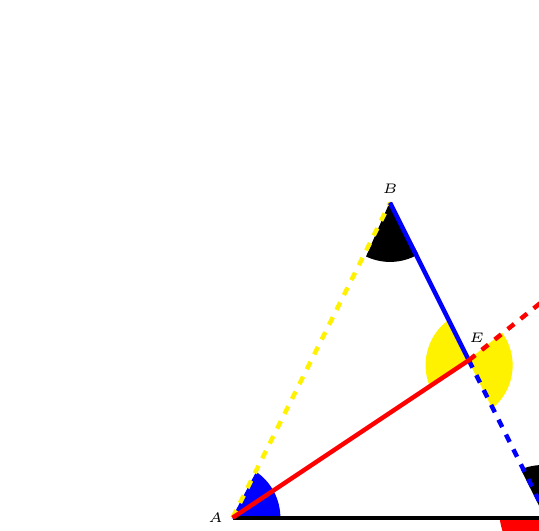
\begin{tikzpicture}
    \draw[blue,fill=blue] (-2, -4) --  (-1.4,-4) arc(0:55:0.7) -- cycle;
    \draw[black,fill=black] (0, 0) -- (0.35, -0.65)  arc(-60:-115:0.7) -- cycle;
    \draw[yellow,fill=yellow] (1, -2) -- (1.3, -2.6)  arc(-50:35:0.7) -- cycle;
    \draw[yellow,fill=yellow] (1, -2) -- (0.5, -2.3)  arc(-160:-235:0.7) -- cycle;
    \draw[red,fill=red] (2, -4) -- (1.4, -4)  arc(185:290:0.7) -- cycle;
    \draw[black, ultra thick,fill=black] (2, -4) -- (1.7, -3.4)  arc(-250: -295: 0.7) -- cycle;
    \draw[black,ultra thick] (2, -4) -- (2.5, -4)  arc(-4:50:0.7) -- cycle;
    
    \draw[dashed, yellow, ultra thick] (-2,-4) --  (0,0);
    \draw[blue, ultra thick] (0,0) --  (1, -2);
    \draw[dashed, blue, ultra thick] (1,-2) --  (2, -4);
    \draw[black, ultra thick] (-2,-4) --  (2, -4);
    \draw[dashed, black, ultra thick] (2,-4) --  (3.5, -4);
    \draw[black, ultra thick] (2,-4) --  (2.75, -5.5);
    \draw[red, ultra thick] (-2,-4) --  (1, -2);
    \draw[dashed, red, ultra thick] (1, -2) --  (3.5, 0);
    \draw[yellow, ultra thick] (3.5, 0) --  (2, -4);
    
    \node[above] at (0,0) {{\tiny$B$}};
    \node[left] at (-2,-4) {{\tiny$A$}};
    \node[below] at (2.3, -4) {{\tiny$C$}};
    \node[above] at (1.1, -1.9) {{\tiny$E$}};
    \node[below] at (3.5, -4) {{\tiny$F$}};
    \node[right] at (2.75, -5.5) {{\tiny$G$}};
    \node[above] at (3.5, 0) {{\tiny$D$}};
    
    \end{tikzpicture}

     \end{center}
\end{minipage}\hfill
\begin{minipage}[t]{0.57\textwidth}
  \Mainclt
  \begin{wrapfigure}{l}{0.2\linewidth}
    \includegraphics[width=0.9\linewidth]{images/П.png}
  \end{wrapfigure}\\
  \slshape ри \textit{продолжении стороны треугольника
  \begin{tikzpicture}
   \draw[dashed, orange, ultra thick] (-0.5,-1) --  (0,0);
    \draw[blue, ultra thick] (0,0) --  (0.25, -0.5);
    \draw[dashed, blue, ultra thick] (0.25,-0.5) --  (0.5, -1);
    \draw[black, ultra thick] (-0.5,-1) --  (0.5, -1);
    \node[above] at (0,0) {{\tiny$B$}};
    \node[left] at (-0.5,-1) {{\tiny$A$}};
    \node[right] at (0.5, -1) {{\tiny$C$}};
  \end{tikzpicture} внешний угол \begin{tikzpicture}
    \draw[black, ultra thick,fill=black] (2, -4) -- (1.7, -3.4)  arc(-250: -295: 0.7) -- cycle;
    \draw[black,ultra thick] (2, -4) -- (2.5, -4)  arc(-4:50:0.7) -- cycle;
    \node[below] at (2, -4) {{\tiny$C$}};
    \node[left] at (1.7, -3.4) {{\tiny$E$}};
    \node[right] at (2.5, -4) {{\tiny$F$}};
  \end{tikzpicture} будет больше любого из противолежащих ему внутренних углов
  \begin{tikzpicture}
  \draw[black,fill=black] (0, 0) -- (0.35, -0.65)  arc(-60:-115:0.7) -- cycle;
   \node[above] at (0,0) {{\tiny$B$}};
    \node[below] at (0.35, -0.65) {{\tiny$C$}};
    \node[below] at (-0.35, -0.65) {{\tiny$A$}};
  \end{tikzpicture} или
    \begin{tikzpicture}
        \draw[blue,fill=blue] (-2, -4) --  (-1.4,-4) arc(0:55:0.7) -- cycle;
        \node[above] at (-1.8, -3.5) {{\tiny$B$}};
        \node[below] at (-2, -4) {{\tiny$A$}};
        \node[below] at (-1.4,-4) {{\tiny$C$}};
    \end{tikzpicture}.}
  
  \upshape
  \begin{center}
   Сделаем
    \begin{tikzpicture}
      \draw[blue,ultra thick] (0,0) -- (1,0);
    \node[above] at (0,0) {{\tiny$B$}};
    \node[above] at (1,0) {{\tiny$E$}};
  \end{tikzpicture}
  $=$
    \begin{tikzpicture}
        \draw[dashed, blue,ultra thick] (0,0) -- (1,0);
        \node[above] at (0,0) {{\tiny$E$}};
        \node[above] at (1,0) {{\tiny$C$}};
    \end{tikzpicture} (пр. I.{\tiny I0}); \\
     проведем
    \begin{tikzpicture}
    \draw[red,ultra thick] (0,0) -- (1,0);
    \node[above] at (0,0) {{\tiny$A$}};
    \node[above] at (1,0) {{\tiny$E$}};
  \end{tikzpicture}
    и продлим до
    \begin{tikzpicture}
      \draw[dashed, red, ultra thick] (0,0) -- (1,0);
    \node[above] at (0,0) {{\tiny$E$}};
    \node[above] at (1,0) {{\tiny$D$}};
  \end{tikzpicture}. 
  $=$
   \begin{tikzpicture}
      \draw[red, ultra thick] (0,0) -- (1,0);
    \node[above] at (0,0) {{\tiny$A$}};
    \node[above] at (1,0) {{\tiny$E$}};
  \end{tikzpicture}. 
    \vspace{0.4cm}
    проведем
    \begin{tikzpicture}
      \draw[yellow,ultra thick] (0,0) -- (1,0);
    \node[above] at (0,0) {{\tiny$C$}};
    \node[above] at (1,0) {{\tiny$D$}};
  \end{tikzpicture}. В 
   \begin{tikzpicture}
    \draw[dashed, yellow, ultra thick] (-0.5,-1) --  (0,0);
    \draw[blue, ultra thick] (0,0) --  (0.25, -0.5);
    \draw[red, ultra thick] (-0.5,-1) --  (0.25, -0.5);
    \node[above] at (0,0) {{\tiny$B$}};
    \node[left] at (-0.5,-1) {{\tiny$A$}};
    \node[right] at (0.25, -0.5) {{\tiny$E$}};
  \end{tikzpicture}  и
  \begin{tikzpicture}
    \draw[dashed, blue, ultra thick] (0.25,-0.5) --  (0.5, -1);
    \draw[dashed, red, ultra thick] (0.25, -0.5) --  (0.75, 0);
    \draw[yellow, ultra thick] (0.75, 0) --  (0.5, -1);
    \node[below] at (0.5, -1) {{\tiny$C$}};
    \node[left] at (0.25, -0.5) {{\tiny$E$}};
    \node[above] at (0.75, 0) {{\tiny$D$}};
  \end{tikzpicture};
  
    \begin{tikzpicture}
      \draw[blue ,ultra thick] (0,0) -- (1,0);
    \node[above] at (0,0) {{\tiny$B$}};
    \node[above] at (1,0) {{\tiny$E$}};
  \end{tikzpicture} =
   \begin{tikzpicture}
    \draw[dashed, blue,ultra thick] (0,0) -- (1,0);
    \node[above] at (0,0) {{\tiny$E$}};
    \node[above] at (1,0) {{\tiny$C$}};
  \end{tikzpicture}, 
  \begin{tikzpicture}
    \draw[yellow,fill=yellow] (1, -2) -- (0.5, -2.3)  arc(-160:-235:0.7) -- cycle;
    \node[above] at (0.9, -1.6) {{\tiny$B$}};
    \node[below] at (0.4, -2.3) {{\tiny$A$}};
    \node[right] at (1, -2) {{\tiny$E$}};
  \end{tikzpicture} $=$
  \begin{tikzpicture}
    \draw[yellow,fill=yellow] (1, -2) -- (1.3, -2.6)  arc(-50:35:0.7) -- cycle;
    \node[below] at (1.4, -2.6) {{\tiny$D$}};
    \node[above] at (1.4, -1.7) {{\tiny$C$}};
    \node[left] at (1, -2) {{\tiny$E$}};
  \end{tikzpicture} \\
  (пр. I.{\tiny5}) и 
  \begin{tikzpicture}
      \draw[red ,ultra thick] (0,0) -- (1,0);
    \node[above] at (0,0) {{\tiny$A$}};
    \node[above] at (1,0) {{\tiny$E$}};
  \end{tikzpicture} =
\begin{tikzpicture}
    \draw[dashed, red,ultra thick] (0,0) -- (1,0);
    \node[above] at (0,0) {{\tiny$E$}};
    \node[above] at (1,0) {{\tiny$D$}};
\end{tikzpicture}  (постр.), 

  $\therefore$
  \begin{tikzpicture}
  \draw[black,fill=black] (0, 0) -- (0.35, -0.65)  arc(-60:-115:0.7) -- cycle;
   \node[above] at (0,0) {{\tiny$B$}};
    \node[below] at (0.35, -0.65) {{\tiny$C$}};
    \node[below] at (-0.35, -0.65) {{\tiny$A$}};
  \end{tikzpicture} = 
  \begin{tikzpicture}
     \draw[black, ultra thick,fill=black] (2, -4) -- (1.7, -3.4)  arc(-250: -295: 0.7) -- cycle;
     \node[above] at (2.3, -3.4) {{\tiny$E$}};
    \node[above] at (1.7, -3.4) {{\tiny$D$}};
    \node[below] at (2, -4) {{\tiny$C$}};
    \end{tikzpicture} (пр. I.{\tiny $4$}), \\
    \begin{tikzpicture}
    \draw[black, ultra thick,fill=black] (2, -4) -- (1.7, -3.4)  arc(-250: -295: 0.7) -- cycle;
    \draw[black,ultra thick] (2, -4) -- (2.5, -4)  arc(-4:50:0.7) -- cycle;
    \node[below] at (2, -4) {{\tiny$C$}};
    \node[left] at (1.7, -3.4) {{\tiny$E$}};
    \node[right] at (2.5, -4) {{\tiny$F$}};
  \end{tikzpicture} $>$ 
  \begin{tikzpicture}
    \draw[black,fill=black] (0, 0) -- (0.35, -0.65)  arc(-60:-115:0.7) -- cycle;
   \node[above] at (0,0) {{\tiny$B$}};
    \node[below] at (0.35, -0.65) {{\tiny$C$}};
    \node[below] at (-0.35, -0.65) {{\tiny$A$}};
    \end{tikzpicture}. \\
  Так же можно показать, что при \\
  продлении \begin{tikzpicture}
    \draw[blue, ultra thick] (0,0) -- (1,0);
    \node[above] at (0,0) {{\tiny$B$}};
    \node[above] at (1,0) {{\tiny$C$}};
\end{tikzpicture}, \begin{tikzpicture}
    \draw[red,fill=red] (2, -4) -- (1.4, -4)  arc(185:290:0.7) -- cycle;
    \node[above] at (2, -4) {{\tiny$G$}};
    \node[below] at (2.3, -4.6) {{\tiny$A$}};
    \node[below] at (1.2,-3.8) {{\tiny$C$}};
\end{tikzpicture} $>$
\begin{tikzpicture}
    \draw[blue,fill=blue] (-2, -4) --  (-1.4,-4) arc(0:55:0.7) -- cycle;
        \node[above] at (-1.8, -3.5) {{\tiny$B$}};
        \node[below] at (-2, -4) {{\tiny$A$}};
        \node[below] at (-1.4,-4) {{\tiny$C$}};
\end{tikzpicture} \\
и, следовательно \begin{tikzpicture}
    \draw[black, ultra thick,fill=black] (2, -4) -- (1.7, -3.4)  arc(-250: -295: 0.7) -- cycle;
    \draw[black,ultra thick] (2, -4) -- (2.5, -4)  arc(-4:50:0.7) -- cycle;
    \node[below] at (2, -4) {{\tiny$C$}};
    \node[left] at (1.7, -3.4) {{\tiny$E$}};
    \node[right] at (2.5, -4) {{\tiny$F$}};
  \end{tikzpicture} который  \\
  = \begin{tikzpicture}
    \draw[red,fill=red] (2, -4) -- (1.4, -4)  arc(185:290:0.7) -- cycle;
    \node[above] at (2, -4) {{\tiny$G$}};
    \node[below] at (2.3, -4.6) {{\tiny$A$}};
    \node[below] at (1.2,-3.8) {{\tiny$C$}};
\end{tikzpicture} будет $>$ \begin{tikzpicture}
    \draw[black,fill=black] (0, 0) -- (0.35, -0.65)  arc(-60:-115:0.7) -- cycle;
   \node[above] at (0,0) {{\tiny$B$}};
    \node[below] at (0.35, -0.65) {{\tiny$C$}};
    \node[below] at (-0.35, -0.65) {{\tiny$A$}};
    \end{tikzpicture}. 
  
  \end{center}
  \begin{flushright}
    ч. т. д.
  \end{flushright}
\end{minipage}
\end{document}